%!TEX root = main.tex
\Lesson{Символы и формальные функции}\label{Less:symbols}

\section{Символы и~их значения}%
До сих пор мы имели дело с~константами и~символами-идентификаторами, игравшими роль переменных или имён функций. При~этом символ должен был быть связан с~каким-либо значением~--- константой или функцией, в~противном случае возникала ошибка.

Если мы собираемся производить символьные преобразования, то нам вовсе не~обязательно требовать чтобы символы имели какие-то конкретные значения. Например, если мы рассматриваем преобразование $(a + b)^2 = a^2 + 2ab + b^2$, нам не~важно, чему равны $a$ и~$b$~--- мы работаем с~формальными символами.

Язык \Scheme позволяет работать с~выражениями, не~вычисляя их. Для этого служит кавычка \s{'} (сокращение для формы \s{quote}\index{Racket!базовые формы!quote@\s{'} (\s{quote})}).

\begin{example}{Попробуем ввести выражение с~неопределёнными символами и~получим сообщение об~ошибке.

Использование формы \s{quote} оставляет выражение невычисленным.}
\REPLin
  {(+ a b)}

\REPLerror{reference to an identifier before its definition: a}

\REPL
  {(quote (+ a b))}
  {(+ a b)}
\end{example}

\begin{example}{%
Знак кавычки \s{'} является кратким обозначением формы \s{quote}:}
\REPL{'(+ a b)}{(+ a b)}
\end{example}

\begin{example}{В то время, как первый элемент списка \s{(list a 'a)} вычисляется, второй остаётся в~виде символа.}
\REPLin
  {(define a 8)}

\REPL
  {(list a 'a)}
  {(8 a)}
\end{example}

Выражение, взятое в~кавычки, можно вычислить с~помощью функции \sbi{eval}:

\begin{example}{Выражение \s{x} содержит в~себе невычисленную сумму. Применение функции \s{eval} снимает кавычки и~вычисляет его, применяя все известные интерпретатору определения.}
\REPLin
  {(define x '(+ a 5))}

\REPL
  {x}
  {(+ a 5)}

\REPL
  {(eval x)}
  {13}
\end{example}

По существу, функция \s{eval} является вызовом интерпретатора \Scheme для введённого выражения:

\begin{example}{Выражение \s{proc} содержит в~себе определение функции.

Это определение не~выполняется,  и~символ \s{1+} является неопределённым.

Функция \s{eval} интерпретирует  выражение \s{proc}, как программу \Scheme.}
\begin{ExampleCode}
(define proc
  '(define (1+ x)
       (+ 1 x)))
\end{ExampleCode}

\REPL
  {proc}
  {'(define (1+ x) (+ 1 x))}

\REPLin
  {(1+ 2)}

\REPLerror{1+: undefined;\newline cannot reference an identifier before its definition}

\REPLin
  {(eval proc)}

\REPL
  {(1+ 2)}
  {3}
\end{example}

Часто бывает нужно оставив выражение невычисленным, вычислить некоторые его части. Для этого служит форма \s{quasiquote} или символ \s{`} (обратная кавычка).\index{Racket!базовые формы!quasiquote@\s{`} (\s{quasiquote})} Эта форма работает так же, как и~\s{quote}, но часть выражения можно заменить его значением, если поместить его в~форму \s{unquote} или поставить перед ним символ \s{,} (запятая).\index{Racket!базовые формы!unquote@\s{,} (\s{unquote})}

\begin{example}{Обратная кавычка позволяет вычислять только ту часть выражения, которая следует за~знаком запятой. Всё остальное остаётся невычисленным.}
\REPL
  {`(a ,(+ 2 3) (+ 1 2))}
  {'(a 5 (+ 1 2))}
\end{example}

\begin{example}{Комбинация символов \s{,@} не~просто вычисляет подвыражение, но и~убирает лишние скобки.}
\REPLin
  {(define x '(a b c))}

\REPL
  {`(+ ,x)}
  {'(+ (a b c))}

\REPL
  {`(+ ,@x)}
  {'(+ a b c)}
\end{example}

Кавычки \s{quote}, \s{quasiquote} и~функция \s{eval} являются мощным инструментом~--- они дают нам способ строить выражения, которые работают с~другими выражениями. Таким образом, в~функциональных языках стирается принципиальное различие между программой и~данными, поскольку данные сами могут играть роль программы.

\section[4]{Эквивалентность констант, символов и~структур}%
Разделение символов и~их значений приводит к~следующему вопросу: в~каких случаях считать эквивалентными символы и~структуры? Пока мы имели дело только с~числовыми константами, нам хватало предиката равенства \s{=}. Для символов и~их значений в~\Scheme существует \emph{предикат эквивалентности} \sbi{equal?}.

Предикат \s{equal?} возвращает \s{#t} если его аргументы являются одинаковыми символами или если они связаны с~одним и~тем же объектом в~памяти, а~также для одинаковых структур с~совпадающими элементами.

\REPL
  {(equal? 1 1)}
  {\#t}

\REPL
  {(equal? (cons 1 2) (cons 1 2))}
  {\#t}

\REPLin{(define a 'b)}
\REPL
  {(equal? (cons a a) (cons 'b 'b))}
  {\#t}

\REPL
  {(equal? 1.0 1)}
  {\#f}

\REPL
  {(equal? '(1 2 ((b) a)) '(1 2 ((b) a)))}
  {\#t} 

\begin{Assignment}
a) Напишите предикат \si{almost-equal?}, который возвращает \s{#t} в~тех же случаях, что и~\s{equal?}, но при~этом, сравнивая числа, считает их равными, если они отличаются только в~14-ой значащей цифре.

\begin{Tip}
Начните выполнение задания с~определения типа и~тестовых примеров для функции!
\end{Tip}

\end{Assignment}

%=============================================================
% Формальные функции
%=============================================================

\section[4]{Абстрактные типы данных и \mbox{формальные~функции}}%
\index{тип!абстрактный}%
На предыдущем занятии мы встретились с понятием абстрактного типа данных. Экземпляры таких типов образуются с помощью функций-конструкторов, не производящих никаких вычислений, и возвращающих данные <<упакованными>> в определённую структуру. Для того чтобы отличать величины принадлежащие разным абстрактным типам, необходим идентификатор типа. Доступ к элементам такой структуры осуществляется функциями-селекторами. Кроме использования функций-селекторов, получить доступ к элементам величины абстрактного типа позволяет техника сопоставления с образцом. Примером абстрактного типа является точечная пара с конструктором \s{cons}, селекторами \s{car} и \s{cdr} и идентифицирующим предикатом \s{pair?} и дескриптором \s{cons:}.


В языке \Scheme для создания новых абстрактных типов служат \index{функция!формальная}\emph{формальные функции}, которые, не~производя никаких вычислений, возвращают в~качестве результата заквотированное выражение, обозначающее их аппликацию.

Объявляются формальные функции формой \sfi{define-formal}.

\begin{example}{%
Декларируем функции \s{f} и \s{g}, как формальные. Причём \s{f} может принимать произвольное количество аргументов, а \s{g} является бинарной. Результатом аппликации формальной функции является список.}
\REPLin
  {(define-formal f (g 2))}
\REPL
  {(f 1)}
  {(f 1)}
\REPL
  {(f (g 'x 'y) 'z)}
  {(f (g x y) z)}
\REPL
  {(is (f 'x) list?)}{#t}
\end{example}

\begin{example}{%
При объявлении формальной функции с сименем \s{id} создаются
\begin{itemize}
\item идентифицирующий предикат \s{id?}, отличающий аппликацию этой функции от других списков, 
\item шаблон для этой функции \s{(id ...)} 
\item и дескриптор для абстрактного типа \s{id:}.
\end{itemize}}
\REPL{(is (f 1) f?)}{#t}
\REPL{(is (f 1) g?)}{#f}
\smallskip
\begin{ExampleCode}
> ((/. (f a b) --> a) 
   (f 1 2))
\end{ExampleCode}
\REPLout{1}
\smallskip
\begin{ExampleCode}
> (is (f (g 1 2) 3)
      (f: (g: Int Int) Int))
\end{ExampleCode}
\REPLout{#t}
\end{example}

\vspace{-\bigskipamount}
\begin{Assignment}
а) Напишите своё простейшее определение формальной функции \s{f}, удовлетворяющей спецификации:
\begin{Specification}
(test 
  (f 'x)                ==> '(f x)
  (f 1 2 3)             ==> '(f 1 2 3)
  (map f '(1 2 3))      ==> '((f 1) (f 2) (f 3)))
\end{Specification}

б) Определите функцию \fun{hold}{s}, которая бы делала формальной функцией любой указанный символ. 
\begin{Specification}
(test 
 ((hold 'g) 1 2 3)             ==> '(g 1 2 3)
 (map (hold '+) '(1 2) '(3 4)) ==> '((+ 1 3) (+ 2 4)))
\end{Specification}

Приведите два варианта определения этой функции: с~использованием форм \s{quote} и~\s{quasiquote} и без них.

\end{Assignment}

%=============================================================
% Пример: расчёт электрических цепей
%=============================================================

\section{Пример: расчёт электрических цепей}%
В качестве развёрнутого практического примера, использования формальных функций для создания абстрактных типов данных, рассмотрим задачу расчёта импеданса электрических цепей переменного тока. Мы будем рассматривать цепи, содержащие только сопротивления, индуктивности и~ёмкости.

Как известно, в~случае переменного тока, каждый из~рассмотренных нами типов элементов имеет полное сопротивление~--- \emph{импеданс} $Z$, выражаемый комплексным числом. Действительная часть этого числа отражает активное сопротивление элемента, а мнимая --- реактивное. Для заданной частоты переменного тока в~цепи $\omega$ импедансы сопротивления $R$, индуктивности $L$, и ёмкости $C$ вычисляются следующим образом:
$$Z_R = R,\qquad Z_C = -\frac{i}{\omega C},\qquad Z_L = i\omega L.$$
Кроме этого, можно вычислить импедансы для последовательного и~параллельного соединения элементов цепи:
$$Z_\text{посл} = \sum\limits_i Z_i,\qquad  Z_\text{парал}= \left(\sum\limits_i\frac1{Z_i}\right)^{-1}.$$

Для представления электрических схем нужна форма записи, как для элементов, так и~для возможных типов их соединения. Мы будем использовать следующие обозначения:

\begin{itemize}
 \item[] \s{(R $x$)} для сопротивления в~$x$ ом;

 \item[] \s{(L $x$)} для катушки индуктивностью $x$ генри;

 \item[] \s{(C $x$)} для конденсатора ёмкостью $x$ фарад;

 \item[] \s{(-- $el_1$ $el_2$ ...)} для последовательного соединения элементов;

 \item[] \s{(|| $el_1$ $el_2$ ...)} для параллельного соединения.
\end{itemize}

Определим для элементов цепи соответствующие формальные функции:
\begin{Definition}
(define-formal 
  (R 1) (C 1) (L 1) -- ||)
\end{Definition}
\noindent Сразу же опишем и тип для корректной электрической цепи, используя дескрипторы созданных нами формальных функций:
\begin{Definition}
(define-type Circuit
  (R: positive?)
  (C: positive?)
  (L: positive?)
  (--: Circuit ..)
  (||: Circuit ..))
\end{Definition}
Так, например, можно представить в~виде символьного выражения цепь $S$, изображённую на~рисунке:

\medskip
\begin{tabular}{lm{0.4\linewidth}}%
\label{S}
\begin{SchemeCode}
(define S
  (-- (R 10)
      (|| (L 0.5e-6)
          (-- (R 3)
              (C 10e-9)))))
\end{SchemeCode}
&
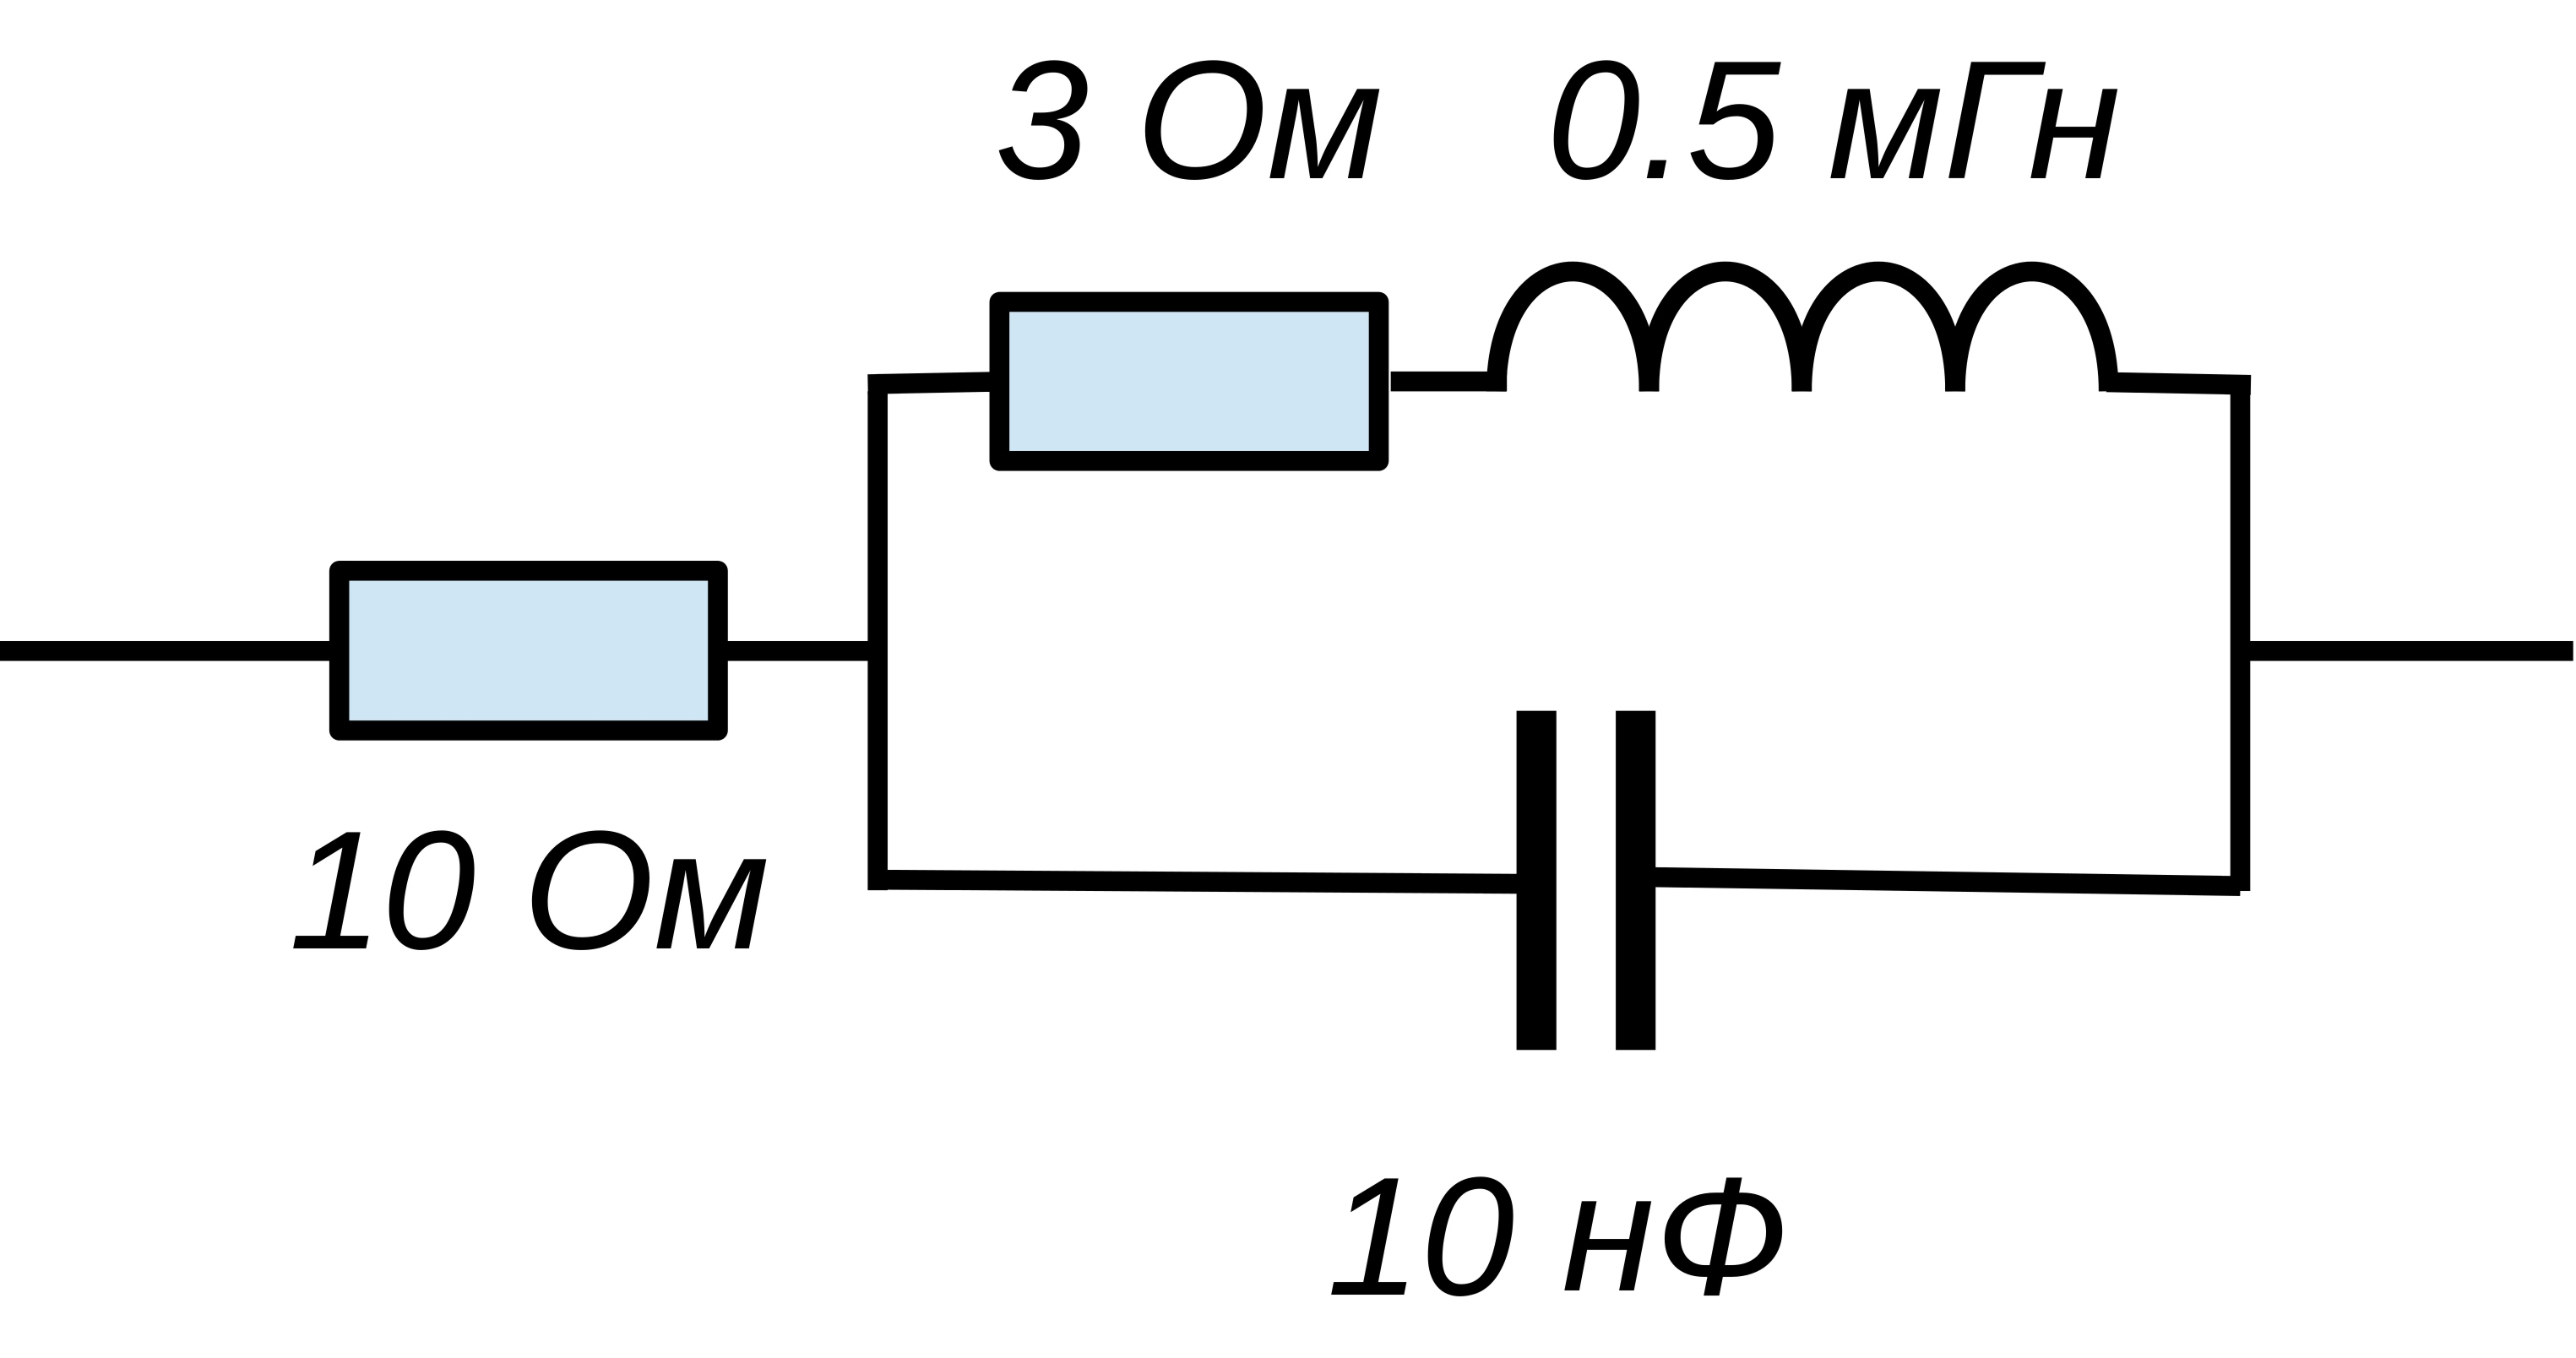
\includegraphics[width=\linewidth]{../figures/circuit.pdf}
\end{tabular}
\vspace{-\medskipamount}
\REPL{S}{'(-- (R 10) (|| (L 5e-06) (-- (R 3) (C 1e-07))))}
\REPL{(is S Circuit)}{#t}
Символьное выражение, описывающее электрическую цепь, представляет собой обыкновенный список. Он может быть создан в программе при помощи формальных функций, а может быть считан из файла <<в готовом виде>>, как любой другой список.

Таким образом, мы определили язык, пригодный для описания простых электрических цепей. Теперь нужно научиться его интерпретировать и производить расчёты. Интерпретатор, который мы хотим создать, должен по заданной цепи строить функцию, вычисляющую импеданс цепи $Z$ для заданной частоты $\omega$. 
Для наглядности, определим типы для этих величин: частота должна быть положительным действительным числом, а импеданс --- комплексным.
\begin{Definition}
 (define-type $\omega$ positive?)
 (define-type Imp complex?)
\end{Definition}
Теперь мы можем записать сигнатуру и <<скелет>> функции\=/интерпретатора \s{impedance} следующим образом:
\label{example:impedance}%
\begin{SchemeCode}[emph={cir,w}]
(:: impedance (Circuit -> ($\omega$ -> Imp))
 (define (impedance cir)
   (lambda (w) ...)))
\end{SchemeCode}

В теле \lmфункции нужно определить, как вычисляются импеданс элементов и соединений. Это нетрудно сделать с помощью сопоставления с образцом. Определим вспомогательную функцию \s{Z}, которая и будет производить это сопоставление:
\begin{Definition}[emph={cir,w}]
(:: impedance (Circuit -> ($\omega$ -> Imp))
 (define (impedance cir)
   (lambda (w) 
     (define/. Z
       (R r) --> r
       (C c) --> (/ -i c w)
       (L l) --> (* +i l w)
       (-- i ...) --> (sum Z i)
       (|| i ...) --> (/ (sum / (map Z i))))
     (Z cir))))

(:: sum ((Any -> Num) list? -> Num)
  (define (sum f lst) 
    (apply + (map f lst))))
\end{Definition}
Здесь мы постарались максимально выразительно указать способ вычисления импеданса соединений через функцию \s[emph={f,lst}]{(sum f lst)}, вычисляющую сумму значений функции \lex{f} на элементах списка \lex{lst}. Внутрення \lmфункция  просто возвращает результат интерпретации входной цепи \lex{cir} функцией \s{Z}.

Теперь всё готово для расчётов:
\REPL
  {((impedance circuit) 1e6)}
  {12.205882352941176+8.676470588235293i}

\begin{Assignment}
а) С помощью функции \s{plot} постройте график модуля импеданса цепи $S$ в диапазоне от 1\,МГц до 50\,MГц.

б) Имея функцию для импеданса какой-либо цепи, мы можем, например, вычислить резонансную частоту цепи, численно решив уравнение $\mathrm{Im} Z(\omega) = 0$.

Напишите функцию \fun{resonant-frequency}{circ $\omega_1$ $\omega_2$}, которая бы находила резонансную частоту для цепи \lex{circ} в~диапазоне частот от~$\omega_1$ до~$\omega_2$. Воспользуйтесь для решения уравнения функцией \s{bisection}, которую мы рассмотрели на~Занятии \ref{Less:recursion}  (стр.\,\pageref{bisection}).

в) Найдите при каком значении ёмкости $C$, резонансная частота цепи $S$, будет равна 20\,MГц. 

Подумайте, как с помощью мемоизации можно ускорить вычисления, не переписывая функции \s{bisection} и \s{impedance}?
\end{Assignment}

\section{Программа, \mbox{управляемая данными}}%
Существует другой весьма изящный, чисто функциональный способ решения рассмотренной нами задачи расчёта электрических цепей. Он основывается на подходе, иенуемом \emph{программированием, управляемым данными} (data-driven programming). В этом подходе стирается грань между данными и программой, так что описание данных и является обрабатывающей их программой.

Как и в предыдущей реализации будем обозначать элементы цепи функциями \s{R}, \s{C} и \s{L}. Но теперь это будут не формальные функции, а функции для расчёта импедансов отдельных элементов электрической цепи:
\begin{Definition}[emph={r,c,l,w}]
(:: R (positive? $\omega$ -> Imp)
  (define (R r w) r))

(:: C (positive? $\omega$ -> Imp)
  (define (C c w) (/ -i c w)))

(:: L (positive? $\omega$ -> Imp)
  (define (L l w) (* +i l w)))
\end{Definition}\newpage
\noindentТаким образом, например, выражение \s{(C 1e-9)} является частично\=/применённой функцией \s{C} и представляет собой функцию, имеющую сигнатуру \s{$\omega$ -> Imp}.

Функции, вычисляющие импедансы для последовательного и параллельного соединений элементов цепи должны оперировать именно такими функциями. Причём они должны комбинировать их так, чтобы в результате вновь получалась функция, пригодная к комбинированию. Ниже дана реализации этих функций, обратите внимание на их тип.
\begin{Definition}[emph={cs,c,w}]
(:: -- (($\omega$ -> Imp) .. -> ($\omega$ -> Imp))
  (define (-- . cs) 
    (lambda (w) (sum (lambda (c) (c w)) cs))))

(:: || (($\omega$ -> Imp) .. -> ($\omega$ -> Imp))
  (define (|| . cs) 
    (lambda (w) (/ (sum (lambda (c) (/ (c w))) cs)))))
\end{Definition}
Здесь мы используем такое же суммирование, как и в предыдущей реализации, но в роли интерпретирующей функции \s{Z} выступают сами комбинируемые функции.

На этом реализация интерпретатора, управляемого данными окончена. Теперь сама схема является функцией, которая <<умеет>> вычислять свой импеданс:

\begin{SchemeCode}
> (define S
    (-- (R 10)
        (|| (L 0.5e-6)
            (-- (R 3)
                (C 10e-9)))))
\end{SchemeCode}
\REPL{S}{<#procedure>}
\REPL{(S 1e6)}{12.205882352941176+8.676470588235293i}

\begin{Assignment}
 С помощью функции \sbi{time}, сравните быстродействие двух рассмотренных нами реализаций: символьной и управляемой данными.

 Какие преимущества даёт использование каждой из них?
\end{Assignment}

\section{Символьные данные \mbox{за~пределами~\Scheme}}%
Символы в~том виде, в~котором мы их использовали и~будем использовать в~наших программах, характерны для \emph{языков символьной обработки данных}. К~ним, в~первую очередь, относятся языки \Lang{SNOBOL, Refal,} \Lisp и~его диалекты.
В семействе языков \Lisp пространство имён и~пространство символов не~разделяются. Идентификатор отличается от~символа только тем, что с~ним связано некоторое значение. Это свойство делает языки семейства \Lisp по-настоящему символьными и~отличает их от~большинства других языков программирования (в том числе и~функциональных), где пространство имён переменных и~пространство символов или строк разделены.

Работа с~символами не~является специфичной для функционального программирования, но многие задачи обработки символьных данных очень изящно решаются именно в~рамках функциональной парадигмы. 

В большинстве языков программирования высокого уровня роль формальных функций играют \emph{структуры} или \emph{записи} --- именованные контейнеры, обеспечивающие доступ к своему содержимому и идентификацию структурированных данных. Однако  формальные функции являются более гибкими: они не регламентируют число и тип полей, хотя и это возможно.

В наибольшей степени, формальные функции, реализованые в \Scheme, соответствуют функциям в языка \Lang{Mathematica}. Там они так же играют роль контейнеров и идентификаторов типа, так же используются для сопоставления с образцом и для символьных вычислений.

В какой-то мере, их использование для определения типов соответствует контрукторам типов в языке \Lang{Haskell}. Существенная разница состоит в том, что в \Scheme формальные аппликации (результат применения формальных функций) представляют собой обыкновенные списки, то есть могут быть созданы любым другим способом или просто считаны из файла, однако их можно обрабатывать, как структурированные и типизированные данные с помощью сопоставления с образцом. В языке \Lang{Haskell} типизированные константы являются объектами более высокого класса.

\newpage
\begin{Queeze}
 \item Какова роль символов в~языке \Scheme?

 \item Каким образом можно создать невычисленное выражение в~языке \Scheme? Как можно вычислить его целиком или частично?

 \item Чтотакое формальная функция и формальная аппликация?
\end{Queeze}
